%!TEX program = xelatex

% -----------------------------------------------------------------------------
% ------------------------------- PREAMBLE ------------------------------------
% -----------------------------------------------------------------------------

\documentclass[english]{scrartcl}

\title{Segregation and Diversity Through an Information Lens} % work on this
\author{\emph{Phil Chodrow}}
\date{\emph{\today}}

\usepackage{pc_writeup}
\usepackage{pc_math}
\usepackage{csvsimple}
\usepackage{subcaption}
\usepackage{csquotes}

\usepackage[colorinlistoftodos]{todonotes}

% -----------------------------------------------------------------------------
% --------------------------------- BODY --------------------------------------
% -----------------------------------------------------------------------------

\begin{document}
\setkomafont{disposition}{\mdseries\rmfamily}

\maketitle

\abstract{}

\section{Introduction} \label{sec:intro}

	% Residential segregation is a persistent fact of modern American cities. Spatial location within cities has been proposed as a generative force of disparity in education and income, as well as mental and physical health \cite{Sharkey2014,DiezRoux2001,Dietz2002,Ludwig2013,Ludwig2012}. Residential segregation -- the differential distribution of different racial groups across urban space -- would then be itself a driver of further inequalities. 

	The quantification of segregation has been a topic of lively conversation within sociology through the last seventy years. This conversation may be coarsely partitioned into two interlocking threads. The first thread concerns the \emph{conceptual dimensions} of segregation, with each dimension reflecting an aspect of the ways in which groups may be separated in space. Most modern authors prefer a subset of the dimensions proposed by Massey and Denton \cite{Massey1988}: evenness, exposure, concentration, centralization, and clustering. Recent writers \cite{Reardon2002,Reardon2004,Roberto2015a,Roberto2015} have tended to focus on the dimensions of evenness and exposure, with \cite{Reardon2004} arguing that the additional clustering and concentration may be considered special cases. 

	The second thread concerns the appropriate methods with which to quantify these dimensions. Most fall into one of two broad classes of mathematical structure.\footnote{These categories are related to but not identical to the standard classification introduced by \cite{Coulter1989}.} \emph{Combinatorial} measures are the most ``physical:'' they measure the probability that two individuals selected under specifiable conditions will fall into two specified racial categories \cite{Goodman1954,James1986}. Combinatorial measures may therefore be intepreted as probabilities of encounters between members of racial groups. They may be differentiated according to the conditions of selection and the choice of categories. Contrasting to combinatorial measures are \emph{information} measures \cite{Theil1971,Theil1967,Roberto2015a}. Information measures are nonphysical in the sense that they do not correspond to probabilities of events. Rather, they reflect an epistemic viewpoint, measuring the ability of an observer to make guesses about individuals' identities when supplied with various kinds of information. Combinatorial and information measures do not exhaust all possibilities, however. For example, \cite{Wong1999} shows that an parametric approach based on the standard deviational ellipses of different groups may also be used to characterize city-scale segregation patterns, and \cite{Osullivan2007} expands this approach using nonparametric methods.

	Theorists have proposed multiple methods for each combination of dimension and mathematical framework, leading to a proliferation of segregation measures. While an abundance of options is in principle a boon to the analyst, relatively little guidance exists on which measures to use \emph{together}.\footnote{\cite{Massey1988} provides some guidance, but this is based on a statistical comparison of a variety measures on data, rather than from first principles.} Some authors use different mathematical paradigms for different dimensions; for example, \cite{Reardon2004} develops a combinatorial approach to evenness and an information theoretic approach to exposure. Considering the intrinsically multidimensional character of segregation itself, a mathematically coherent ensemble of measures is called for. This essay therefore advocates an approach to the study of residential segregation that is \emph{conceptually multidimensional}, \emph{computationally practical}, and \emph{mathematically unified}. 

	\textbf{Conceptually multidimensional.} ``Segregation'' is not a single quantifiable number; it is an intrinsically multidimensional phenomenon that therefore requires a coordinated ensemble of distinct measures. As far as possible, each measure should correspond to exactly one dimension of segregation. Furthermore, each measure should be interpreted in the context of each of the others. In this essay, we adopt the categories of evenness and exposure as emphasized by \cite{Reardon2004}, to which we add the dimension of global diversity of the city as a whole. 

	\textbf{Computationally practical.} Writing in 2004, the authors of \cite{Reardon2004} observe that 
	\begin{displayquote}
		
		[a]t present, few of the proposed spatial segregation measures have been used in published empirical segregation research. These measures have been ignored in part because they typically are more difficult to compute than the aspatial measures.
	
	\end{displayquote}
	Over a decade later, computing resources have expanded dramatically in capability and accessibility. While our focus in this essay is theoretical, our ultimate goal is to place effective tools in the hands of practitioners. To this end, we emphasize interpretability, performance, and ease-of-use in the methods we develop. All are freely available as a package for the \texttt{R} programming language, as described in the Appendix. 

	\textbf{Mathematically unified.} In the measurement of segregation, we typically treat a city as a collection of different types of individuals, distributed differentially in space. The distinct dimensions of segregation correspond to the distinct questions we can ask about these distributions. Information theory is the mathematical framework most suited for the comparison of distributions. Rather than developing  measures for each dimension separately, we show how that an information-theoretic framework leads naturally to an ensemble of conceptually coherent, interpretable metrics resting on a shared mathematical foundation. 

	Our original contribution to this program has three components. The first is a novel measure of spatial exposure -- the local information -- and prove some of its properties. As we show, the local information distinguishes cities with starkly separated monoracial regions from cities with more complex patchwork patterns of racial difference. We argue that the local information, together with global entropy and mutual information, constitute a coherent ensemble of measures for the multidimensional quantification of residential segregation. The second is a novel, information-based algorithm for identifying the spatial structure of residential segregation. The algorithm clusters urban areas into regions whose demographics are relatively constant in space, allowing the analyst to study organic, demographically coherent regions rather than the partially-arbitrary tract or blockgroup demarcations provided by the U.S. Census. The third contribution is to share the tools we develop freely with practitioners: our suite of information measures and our clustering tools are available as open-source software for the \texttt{R} statistical programming language. 

\section{Information and Segregation} \label{sec:information}
	Information theory has long been a mainstay of engineering, computer science, and the natural sciences. Somewhat more recently, information theory has found application in the study of urban phenomena. Theorists have used information measures to have been used to estimate the distribution of populations and resources in space \cite{Webber1979}, guide urban zoning decisions \cite{Batty1972}, identify spatial hierarchies in population distributions \cite{Batty1974,Batty1976}, and measure the complexity of urban phenomena \cite{Bettencourt2015,Batty2014a}. In this section, we develop some key information theoretic concepts and relate them to the dimensions of residential segregation.

	Information theory quantifies structure through an epistemic framework. The core insight is that systemic structure enables \emph{prediction}, while systemic variability can make such prediction difficult. Two systemic features are related when knowledge of one enables better prediction of the other. We can formalize the idea of prediction by considering the following ``guessing game.'' We discuss the weather, and I ask you to give me a \emph{predictive distribution} on the question of whether or not it will rain tomorrow. For example, you might tell me your predictive distribution $p$, where $p(\text{Rain}) = 70\%$ $p(\text{No Rain}) = 30\%$. Tomorrow evening I give you a reward $R(p,W)$ based on your predictive distribution $p$ and the observed weather $W$. For this game to be a true ``guessing game,'' we would expect the function $R$ by which I reward your guess to possess the following intuitive properties: 
	\begin{enumerate}
		\item \textbf{Honesty:} The reward function $R$ encourages you to report your true beliefs about the rain.
		\item \textbf{Fairness:} The reward $R(p,W)$ you receive depends only on your prediction $p$ and the observed outcome, not ``what could have happened.''\footnote{An ``honest'' and ``fair'' reward function is more standardly called ``proper'' and ``local'' among information theorists. 
		}
		\item \textbf{Smoothness:} Your reward increases smoothly as a function of the probability you assigned to the observed outcome. 
	\end{enumerate}
	It is possible to show that these properties uniquely determine the logarithmic reward function $R(p,W) = \log p(W)$ up to an affine transformation.\footnote{\cite{Cover1991,Csiszzr2004}} This logarithmic reward is therefore a fundamental unit of information-theoretic analysis. It is traditional to focus on the negative of the reward function -- the \emph{loss function} $L(p,W) = - R(p,W)$. Large loss reflects to poor prediction. Systemic structure is present when knowledge of a system feature enables us to decrease the loss in such a guessing game. 

	\subsection{Entropy and Global Diversity}

		Consider the following predictive guessing game. You and I are jointly studying residential segregation in Atlanta. I pick a person at random from the city, and ask you to give predictive distribution on their race $Y$, where $Y$ takes possible values in the alphabet  $\mathcal{Y} = \{\text{Asian, Black, Hispanic, Other, White}\}$. There is a true distribution $p(Y)$ corresponding to the proportions of each race in the city in question; in Atlanta in 2014 this true distribution is 
		\begin{align*}
			p(\text{Asian})    &= 6\% \quad
			p(\text{Black})    = 47\% \quad
			p(\text{Hispanic}) = 9\% \\
			p(\text{Other})    &= 4\% \quad
			p(\text{White})    = 35\%\;. 
		\end{align*}
		It is possible to show that your optimal guess in our game is precisely this distribution $p$. Your optimal expected loss is therefore
		\begin{equation*}
			\E_Y[L(p,Y)] = -\E_Y[R(p,Y)] = -\E_Y[\log p(Y)] \triangleq H(Y), 
		\end{equation*}
		where $\E_Y$ is the expectation or averaging operator with respect to $Y$. $H(Y)$ is the Shannon \emph{entropy} of $p$ \cite{Shannon1948}. Throughout this paper logarithms will use the natural base $e = 2.718\ldots$, in which case all information measures have dimensionless units of nats. 

		\begin{figure}
			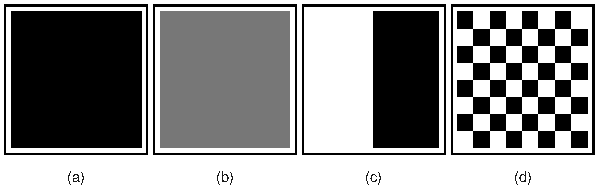
\includegraphics[width=\textwidth]{figs/checkerboard.pdf}
			\caption{Schematic cities illustrating three dimensions of segregation. City (a) lacks global diversity, while Cities (b)-(d) are maximally globally diverse. City (b) is perfectly spatially even, whereas Cities (c) and (d) are maximally uneven. City (d) has higher spatial exposure than City (c) due to more contact points between racially distinct neighborhoods.}. \label{fig:checkerboard}
		\end{figure}

		The Shannon entropy is a natural measure of the global diversity of a city. When $H(Y)$ is low, guessing a randomly-chosen individual's race is easy. An extreme example of this case is when $H(Y) = 0$; in this case, the true distribution $p(Y)$ is unity for one race and zero for the others; i.e. the city is monoracial. Figure \ref{fig:checkerboard}(a) illustrates this case in a schematic two-race city. Perfect prediction without loss is possible because this city lacks diversity. On the other hand, when $H(Y)$ is high, guessing a randomly-chosen individual's race is difficult. An extreme example of this case is when $H(Y)$ achieves its maximum value of $\log \abs{\mathcal{Y}}$, in which case each race is represented equally. The cities in Figure \ref{fig:checkerboard}(b)-(d) all have maximum demographic entropy. The underlying distribution gives you no grounds on which to add probabilistic weight to one race over another; flip a fair coin. Prediction is difficult because of the city's diversity. 

	\subsection{Mutual Information and Spatial (Un)evenness}

		The authors of \cite{Reardon2004} define spatial evenness as ``the extent to which groups are similarly distributed in residential space.'' \emph{Un}evenness, then, is the extent to which these groups are dissimilarly distributed in space. This physical description has an epistemic analogue. In an uneven city, knowing where a resident lives conveys information about their race, in the sense of enabling better prediction. To quantify this intuition, consider two versions of the guessing game in Atlanta. In the first version, I simply choose a random resident and ask you to guess as before. In the second, I choose a random resident but then tell you their location of residence. In the presence of unevenness, this will generally enable you to improve your predictions. For example, in Atlanta knowing that the resident lives in the predominantly white northern part of the city may substantially change your predictive distribution. We can quantify the value of this information as follows. Let $X$ be a random variable denoting the spatial residence. Then, your expected loss in the first game is still $H(Y)$, and your expected loss in the second is $H(Y|X) \triangleq -\E_{Y}[\log p(Y)|X]$. The \emph{mutual information} $I(X,Y)$ is the predictive improvement associated with my telling you the residence: 
		\begin{equation*}
			 I(X,Y) \triangleq H(Y) - H(Y|X)\;.
		\end{equation*}
		Since knowing $X$ can only improve prediction, $I(X,Y) \geq 0$. Furthermore, it is possible to show that 
		\begin{equation}
			I(X,Y) = D[p(X,Y)\|p(X)p(Y)]\;, \label{eq:info_and_divergence}
		\end{equation}
		where 
		\begin{equation*}
			D[q\|r] \triangleq \sum_a q(a) \log \frac{q(a)}{r(a)}
		\end{equation*}
		is the Kullback-Leibler (KL) divergence of $r$ from $q$. Though not an axiomatic metric, the KL divergence may be viewed as a measure of distance between two distributions. Equation \eqref{eq:info_and_divergence} thus shows that the mutual information $I(X,Y)$ can be viewed as the distance of the true joint distribution $p(X,Y)$ of location and race from the hypothetical distribution $p(X)p(Y)$ in which location and race are independent. $I(X,Y)$ therefore measures the degree of dependence between these variables. In this sense, it resembles a correlation coefficient, but has the stronger property that $I(X,Y) = 0$ implies true statistical independence. 

		The mutual information can be viewed as a measure of spatial unevenness (\cite{Roberto2015a}). To see why the mutual information should measure unevenness, consider first the case in which $I(X,Y) = 0$. Since $X$ and $Y$ are independent, knowledge of $X$ does not improve your ability to guess $Y$. City (b) in Figure \ref{fig:checkerboard} illustrates this situation; since ``everywhere is the same,'' location knowledge is of no predictive value. If we were playing in City (b), your performance in the second guessing game would then be equal to your performance in the first. Physically, this situation corresponds to perfect evenness: the distribution of races is $p(Y|X)$ is the same at every location $X$. In contrast, when $I(X,Y)$ achieves its maximum value of $H(Y)$, $X$ fully determines $Y$. This case is illustrated by Figure \ref{fig:checkerboard}(c); if I tell you that a resident lives in the left- or right-hand side of the city, you can guess their race with perfect accuracy. Every location is monoracial, reflecting maximal sociospatial unevenness. 
		
	\subsection{Spatial Exposure}

		The authors of \cite{Reardon2004} define \emph{spatial exposure} as ``the extent that members of one group encounter members of another group...in their local spatial environments.'' We can construct an epistemic analogue of spatial exposure by considering the following pair of guessing games in Atlanta. In each, I pick a resident at random from a small neighborhood that we both know in advance. In the first game, I then ask you to guess that resident's race immediately. In the second, I tell you where \emph{within that neighborhood} the resident lives. If the neighborhood in question is $B$, then your expected loss in the first game is $H(Y|X\in B)$ and in the second $H(Y|X, X\in B)$. The predictive improvement associated with knowing residence within this neighborhood is therefore
		\begin{equation*}
			I(X,Y | X \in B) = H(Y|X\in B) - H(Y|X, X\in B)\;.
		\end{equation*}
		The measure $I(X,Y|X \in B)$ -- the \emph{local (mutual) information} -- is a measure of spatial exposure \emph{in unevenly distributed populations}. This qualification is important, since in a perfectly even population such as Figure \ref{fig:checkerboard}(b),  $I(X,Y) = 0$ and $I(X,Y|X\in B) = 0$ as well. Consider, however, the two unevenly distributed populations in Figure \ref{fig:checkerboard} (c) and (d). In \ref{fig:checkerboard}(c), if we play our two guessing games at a locale entirely within the left- or right-hand halves, the population is locally homogeneous and you can make perfect predictions regardless of the specific residence. Only if we play the game on a locale straddling the middle boundary between the two groups does knowing a resident's specific residence help you to make predictions. If $B$ perfectly straddles the boundary, so that the population proportions are $(\frac{1}{2},\frac{1}{2})$, then we have $H(Y|X\in B) = \log 2$ and $H(Y|X,X\in B) = 0$, so $I(X,Y|X \in B) = \log 2$. 

		This example illustrates that the local information $I(X,Y|X\in B)$ is high when $B$ is an area of demographic transition. When two cities are similarly uneven (have similar $I(X,Y)$), a city with more such transitional areas has more exposure between groups, since residents of one area are closer to demographically different residents of another area. To illustrate, the city of Figure \ref{fig:checkerboard}(d) has the same level of spatial unevenness as \ref{fig:checkerboard}(c), but greater spatial exposure. 

		For practical data analysis, it is necessary to understand how the value of $I(X,Y|X \in B)$ depends on the choice of the locale $B$. In particular, we should expect that when using fine-grained data and fine-grained spatial locales, our estimates of $I(X,Y|X \in B)$ should converge, and not vary wildly as we increase the resolution of our analysis. It is possible to prove mathematically that this is indeed the case. The full proof is given in the appendix, but the idea of the proof is illustrative of the nature of the local information. It begins by noting that the local information is zero on areas of constant demographic structure, but achieves high values in transitional areas. In this sense it behaves like a mathematical derivative. Making this precise requires that we postulate a metric space $M$ and a \emph{probability field} $p(Y|X)$, $X \in M$ with the following properties: 
		\begin{enumerate}
		 	\item $p(y|x) > 0$ for all $x \in M$
		 	\item $p(y|x)$ is differentiable as a function of $x$ for all $x \in M$ and $y \in \mathcal{Y}$. 
		\end{enumerate}
		The probability field $p(y|x)$ corresponds to an idealization of our data; it can be viewed as an interpolation or approximation to the true data using a smooth function. 

		Define $I_r(x)$ to be the local information in a locale of radius $r$ around the point $x$:
		\begin{equation*}
			I_r(x) = I(X,Y| \norm{X - x}^2 \leq r^2). 
		\end{equation*}
		We may view $r$ as the resolution of our analysis. Under the stated conditions, the following approximation relationship holds: 
		\begin{equation}
			\lim_{r \rightarrow 0} \frac{I_r(x)}{r^2} = \frac{1}{4} \text{tr } J_Y(x), \label{eq:fisher_approx}
		\end{equation}
		where $J_Y(x)$ is the \emph{Fisher information in $Y$ about $x$}. It is a matrix defined by the formula
		\begin{equation*}
			J_Y(x) \triangleq \E_Y\left[\nabla_x \log p(Y|x) \left(\nabla_x \log p(Y|x)\right)^T \right]\;. 
		\end{equation*}
		The trace $\text{tr }J_Y(x)$ is the sum of the diagonal entries of $J_Y(x)$. 

		Equation \eqref{eq:fisher_approx} implies that, for small $r$, the local information in a neighborhood of radius $r$, when normalized by $r^2$, is approximately a constant that is independent of $r$. Furthermore, that constant is related to the derivatives of the probability field $p(Y|X)$. We can make this relationship more explicit by noting that 
		\begin{equation}
			\text{tr }J_Y(x) = \E_Y\left[\norm{\nabla_x \log p(Y|x)}^2\right]\;, \label{eq:derivative}
		\end{equation}
		which together with \eqref{eq:fisher_approx} shows that $I_r(x)$ is proportional to the mean magnitude of the derivative of $p(Y|X)$ evaluated at $X = x$.

		In the idealized mathematical framework, we may define the \emph{mean local information} as the average value of the trace of the Fisher information: 
		\begin{equation*}
			J(X,Y) \triangleq \E_X[\text{tr } J_Y(X)].
		\end{equation*}
		Using the relationship \eqref{eq:derivative}, we can recognize $J(X,Y)$ as the total variation of $\log p(Y|X)$ with respect to the probability measure induced by $X$. Intuitively, this is the average ``curviness'' of the field $p(Y|X)$. 

		The measure $J(X,Y)$ may be easily adapted for practical computation. The procedure is as follows:
		\begin{enumerate}
		 	\item Partition the city under analysis into spatial locales $\{B_i\}$.
		 	\item Compute the local information $I(X,Y|X \in B_i)$ for each $i$. 
		 	\item Average the results, weighted by the population of each $B_i$. 
		\end{enumerate} 
		The explicit formula is 
		\begin{align}
			J(X,Y) &= \E_B[I(X,Y|X \in B)] \\ 
			       &= \sum_i p(X \in B_i) I(X,Y|X \in B_i). \label{eq:formula}
		\end{align}
		While the result \eqref{eq:fisher_approx} guarantees limiting resolution-independence in a mathematically idealized setting, in practice it is advisable to use locales $B_i$ of constant size and shape for all regions of analysis. 
	
	\subsection{The Spatial Hierarchy of Measures}
		The information measures we have developed form a natural spatial hierarchy. We can write each using the KL divergence:
		\begin{align}
			H(Y) &= \log \mathcal{\abs{Y}} - D[p(Y) \| u(Y)] \;, \label{eq:H_div} \\ 
			I(X,Y) &= \E_X[D[p(Y|X)]\| p(Y)] \;, \label{eq:I_div} \\ 
			J(X,Y) &= \E_B,X[D[p(Y|X, X\in B) \| p(Y|X \in B)]] \;, \label{eq:J_div}
		\end{align}
		where $u(Y)$ is the uniform distribution on $\mathcal{Y}$. These formulae express each information measure as a divergence or average of divergences. Recalling that a divergence may be viewed as a distance in information space, the formulae make explicit the \emph{comparative} structure of the metrics. The entropy $H(Y)$ is a global measure because it compares the observed global distribution $p(Y)$ to a theoretical global measure, the uniform distribution $u(Y)$. The mutual information $I(X,Y)$ may similarly be viewed as a comparison between the local distribution $p(Y|X)$ and the global distribution $p(Y)$, making it a partially local and partially global metric. On the other hand, the mean local information is a strictly local measure, in the sense that its value depends only on comparisons between two local distributions $p(Y|X,X\in B)$ and $p(Y|X \in B)$, each of which express information only in the locale $B$. The three measures thus sort naturally into a spatial hierarchy, from purely global to purely local. A summary of this hierarchy is given in Figure \ref{fig:hierarchy}. 

		\begin{figure}
			\centering
			\begin{tabular}{l l l l l }
				\textbf{Measure} & \textbf{Comparison type} & \textbf{Compares} & \textbf{To} \\
				\hline 
				 $H(Y)$ & Global-Global & $p(Y)$ & $u(Y)$ \\
				 $I(X,Y)$ & Local-Global & $p(Y|X)$ & $p(Y)$ \\
				 $J(X,Y)$ & Local-Local & $p(Y|X, X \in B)$ & $p(Y|X \in B)$ 
			\end{tabular}
			\caption{Spatial hierarchy of information measures. Each measure can be expressed as an average of comparisons of distributions via the KL divergence \eqref{eq:H_div}-\eqref{eq:J_div}. $u(Y)$ denotes the uniform distribution on $\mathcal{Y}$.} \label{fig:hierarchy}
		\end{figure}


	\subsection{Illustrations}
<<<<<<< HEAD
		% \subsubsection{Comparative Analysis: Detroit and Philadelphia}
			To illustrate these methods, we use them to compare the cities of Philadelphia and Detroit. Our data is blockgroup-level demographics from the American Community Survey \cite{CensusRace}. As we show, computing $H(Y)$, $I(X,Y)$, and $J(X,Y)$ together highlights similarities and differences between these cities. 
			% \todo{We need to generate a nice summary plot here and then fill this section in.}
			\begin{figure}
				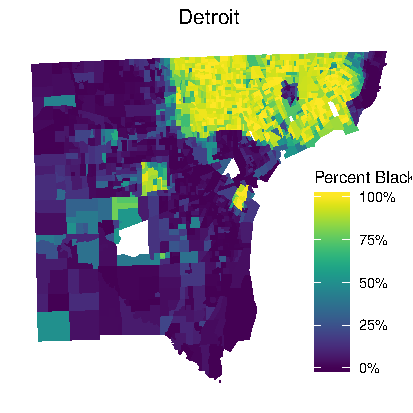
\includegraphics[width = .5\textwidth]{figs/Detroit_percent_black.pdf}
				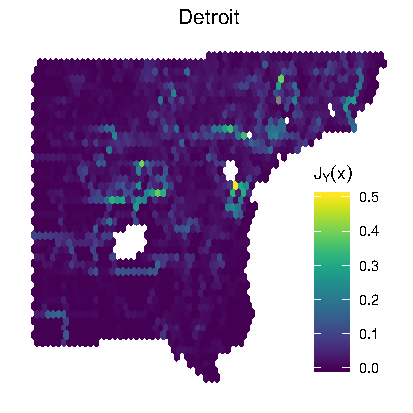
\includegraphics[width = .5\textwidth]{figs/Detroit_grid.pdf} \\
				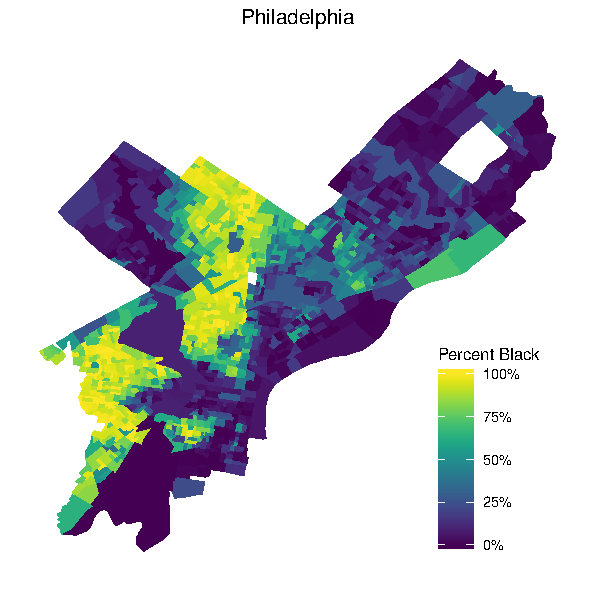
\includegraphics[width = .5\textwidth]{figs/Philadelphia_percent_black.pdf}
				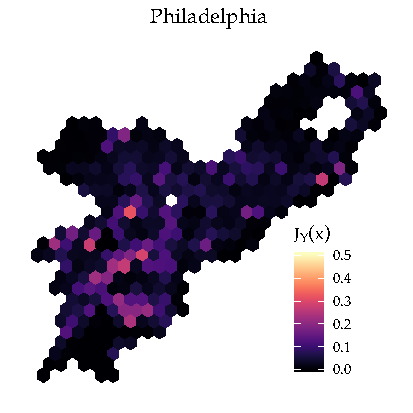
\includegraphics[width = .5\textwidth]{figs/Philadelphia_grid.pdf} \\
=======
		
		\begin{figure}
			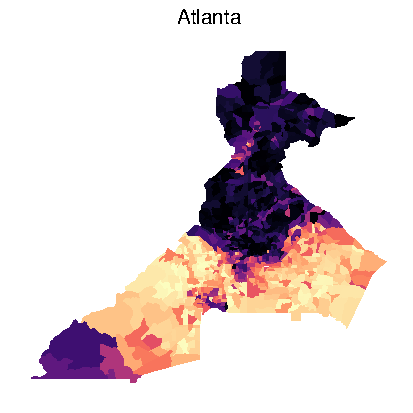
\includegraphics[width = .5\textwidth]{figs/Atlanta_percent_black.pdf}
			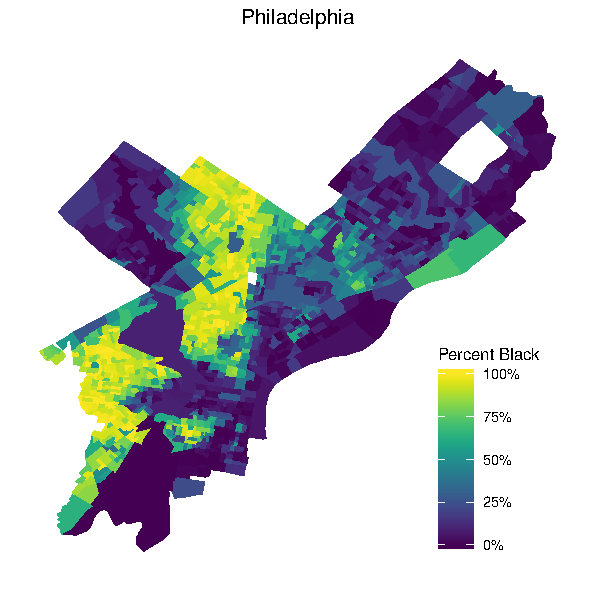
\includegraphics[width = .5\textwidth]{figs/Philadelphia_percent_black.pdf} \\
			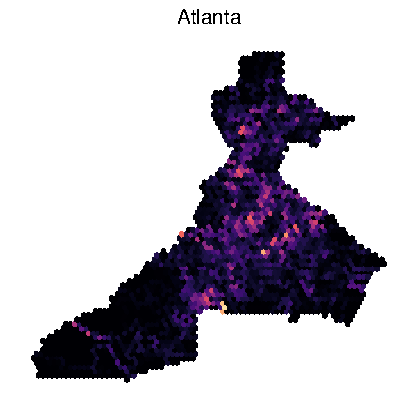
\includegraphics[width = .5\textwidth]{figs/Atlanta_grid.pdf} 
			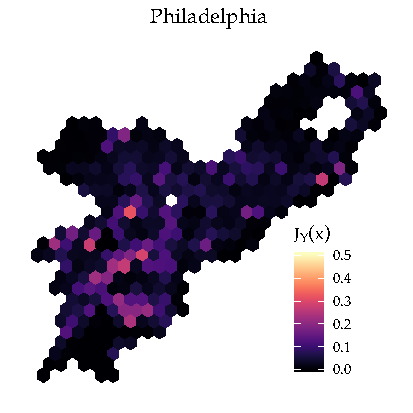
\includegraphics[width = .5\textwidth]{figs/Philadelphia_grid.pdf} \\
>>>>>>> 5f104e78623861e80c09faadeeae9579d0cc0598

			\centering
			\begin{tabular}{l | c c c c}
				\bfseries City & Percent Black & $H(Y)$ & $I(X,Y)$ & $J(X,Y)$  \\\hline
				\csvreader[late after line=\\]{figs/comparative_summary.csv}{}
				{\csvcoli & \csvcolii & \csvcoliii & \csvcoliv & \csvcolv}
			\end{tabular}

			\caption{Spatial analysis of residential segregation in Atlanta (left) and Philadelphia (right). (\emph{Top}): Percentage of black residents. (\emph{Middle}): Hexgrid of spatial resolution 1km imposed over each city, shaded by the value of the local information $I(X,Y | X \in B_i)$. (\emph{Bottom}): Numerical summary, including the three information measures.} \label{fig:Atlanta_philly}
		\end{figure}

<<<<<<< HEAD
		% \subsubsection{Comparative Diversity Profiles}
			% \todo{Is there a fun way to explore the density point? E.g. figure out people per ``neighborhood'' in some way? Think about what I would want the analysis here to be.}
=======
		To illustrate these methods, we use them to compare spatial patterns of segregation in Atlanta and Philadelphia. Our data is blockgroup-level demographics from the American Community Survey \cite{CensusRace}. For visualization purposes, we use the racial categories $\mathcal{Y} = \{\text{Black}, \text{Non-Black}\}$, though we emphasize that these methods generalize to an arbitrary number of categories. Figure \ref{fig:Atlanta_philly} shows the stages of the analysis. First, we visualize the base demographics in space. We then partition each city using a hexagonal grid of radius 1km, and compute the local information within each hexagon. The mean local information $J(X,Y)$ is the average of these local informations. The entropy $H(Y)$ and $I(X,Y)$ do not require spatial computation and can be derived from the cross-tabulation of race by blockgroup. 
		
		One quantitative difference is striking: while Atlanta and Philadelphia are approximately as globally diverse as measured by the entropy $H(Y)$, and approximately as uneven as measured by the mutual information $I(X,Y)$, they vary substantially in their degree of spatial exposure as measured by the mean local information. This quantitative difference reflects the qualitatively distinct patterns of clustering in each city. While Atlanta consists essentially of a northern, predominantly white cluster and a southern, predominantly black one, Philadelphia includes at least three visually distinct clusters with large proportions of black residents. This greater number of clusters generates more sociospatial transitions, which are highlighted by the local information. We will return to the relationship between the local information and clustering in Section \ref{sec:id}. 
>>>>>>> 5f104e78623861e80c09faadeeae9579d0cc0598

		\begin{figure}
			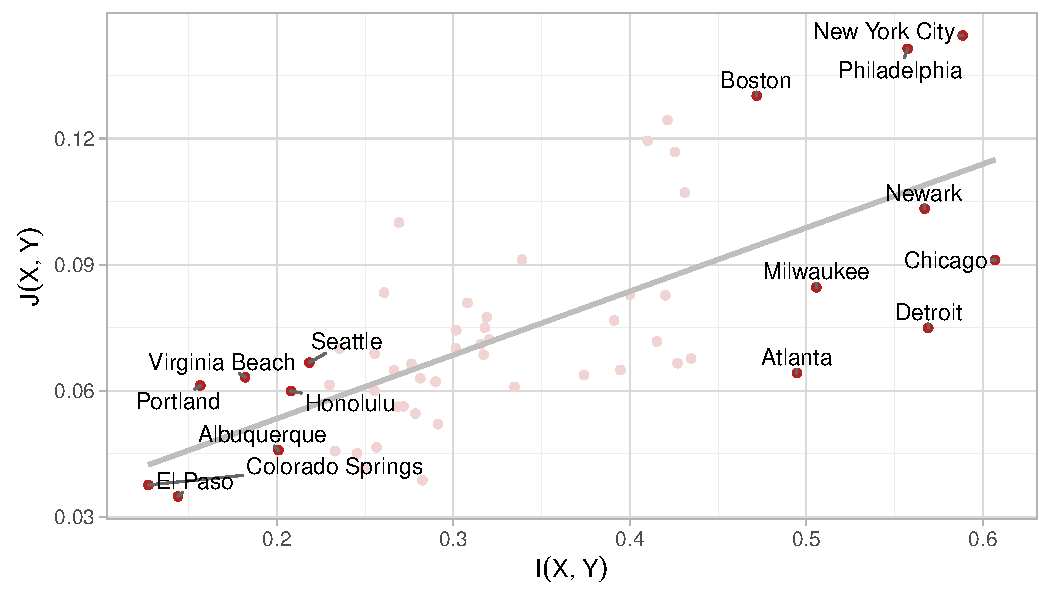
\includegraphics[width=\textwidth]{figs/mutual_fisher.pdf}
			\caption{Comparative global segregation measures in major U.S. cities, measured using racial categories $\mathcal{Y} = \{\text{Asian }, \text{Black }, \text{Hispanic }, \text{Other }, \text{White}\}$. We used a hexgrid of spatial resolution $r = 1$km for the computation of $J(X,Y)$.} \label{fig:mutual_fisher}
		\end{figure}

		We can view Atlanta and Philadelphia in broader context by comparing $I(X,Y)$ and $J(X,Y)$ across a range of American cities in Figure \ref{fig:mutual_fisher}. For each city, we computed $J(X,Y)$ using a 1km hexgrid and the racial categories $\mathcal{Y} = \{\text{Asian}, \text{ Black}, \text{ Hispanic}, \text{ Other}, \text{ White}\}$. The result provides an intuitive sorting of major cities into three overall profiles. Cities toward the bottom left of Figure \ref{fig:mutual_fisher} are relatively spatially even. Cities toward the bottom right, such as Atlanta and Detroit, are highly segregated, with large, starkly separated monoracial regions. Cities toward the top right like Philadelphia and New York are more complex patchworks of smaller, ethnically distinct subregions.  

		


\section{The Spatial Structure of Segregation} \label{sec:id}
	

	The measures $H(Y)$, $I(X,Y)$, and $J(X,Y)$ quantify the presence of different forms of sociospatial structure. In practical analysis, we may wish not only to measure the quantity of structure, but to identify and visualize that structure directly. While approaches exist to this problem,\footnote{For three, see \cite{Logan2011}} these approaches tend to conceptualize this structure in terms of monoracial subregions. In practice, however, there may be coherent biracial or multiracial patterns in space. Fortunately, it is possible to motivate a structure-finding algorithm for identifying high-level demographic trends without restriction to monoracial regions. 

	The key property we will use is ``additive spatial decomposition'' \cite{Reardon2004}. A segregation measure satisfies additive spatial decomposition when, if spatial units are aggregated into groups, the measure can be expressed as a sum of a ``within group'' term expressing variability within aggregations, and a ``between group'' term expressing variability across aggregations. The mutual information $I(X,Y)$ satisfies this property due to the following information-theoretic identity. Let $C$ be a random variable with the property that $H(C|X) = 0$; i.e. $X$ completely determines $C$. We can think of $C$ as group labels for the spatial locations $X$. Then, the chain rule of information\footnote{See \cite{Cover1991}} implies that 
	\begin{equation}
		I(X,Y) = \underbrace{I(C,Y)}_{\text{between-group}} + \underbrace{I(X,Y|C)}_{\text{within-group}}. \label{eq:chain_rule}
	\end{equation}
	Equation \eqref{eq:chain_rule} expresses the following intuitive information decomposition: the information you have if I tell you a person's residence about their race is just the same as the information you would have if I told you first their approximate neighborhood $C$ and then their exact residence $X$. 

	Equation \eqref{eq:chain_rule} motivates a natural algorithm for identifying sociospatial structure. The core idea is that a clustering $C$ is ``good'' when it captures most of the intrinsic information in the system in the between-groups term $I(C,Y)$. This idea is analogous to between-group sum-of-squares maximization in classical k-means clustering. We can also think of it using the standard framework of predictive games discussed in Section \ref{sec:information}. Recall the mutual information game, in which I choose a random resident in Atlanta and tell you their blockgroup of residence. Let us modify the game: instead of telling you one of the blockgroups, I will instead tell you one of $N$ \emph{regions}, each consisting of many blockgroups, for some fixed $N$. Before playing, I give you the opportunity to choose what these regions will be. Some regional divisions will be more useful than others. Suppose, for example, that we are playing this game in Atlanta and $N = 2$. Clearly, knowing whether a resident comes from the northern or southern part of the city is much more predictively valuable than knowing whether that same resident comes from the eastern or western part. You may therefore optimize your performance in our predictive guessing game by choosing to aggregate blockgroups into northern and southern regions. 

	Mathematically, this corresponds to maximizing $I(C,Y)$ subject to a fixed number of clusters. In full generality, this is a challenging discrete optimization problem that may not be computationally tractable. We can, however, construct a greedy algorithm that produces useful results. We begin with the full set of blockgroups. At each stage of the algorithm, we consider the problem of choosing a pair of locales $\{i*, j*\}$ to aggregate together. A good choice of locales leads to minimal information loss, which we may quantify as follows. The mutual information over the full complement $\mathcal{K}$ of blockgroups may be written: 
	\begin{align*}
	 	I(X,Y) &= \sum_{k \in \mathcal{K}} p(X = k) D[p(Y|X = k\|p(Y)] 
	\end{align*} 
	The contribution of locale $k$ to this sum is 
	\begin{align*}
		I_{k}(X,Y) &\triangleq p(X = k)D[p(Y|X = k)\|p(Y)], 
	\end{align*}
	with which notation we may write 
	\begin{equation*}
		I(X,Y) = \sum_{k} I_k(X,Y).
	\end{equation*}
	If we replace $i$ and $j$ with an aggregated local $i\cup j$, its contribution to the mutual information is 
	\begin{align*}
		I_{i\cup j}(X,Y) = p(X \in \{i,j\}) D[p(Y|X \in \{i,j\}) \| p(Y)]\;.
	\end{align*}
	The loss associated with aggregating $i$ and $j$ is the difference between individual contribution and  aggregated contributions:
	\begin{align*}
		d(i,j) \triangleq I_{i}(X,Y) + I_{j}(X,Y) - I_{i \cup j}(X,Y).  
	\end{align*}
	In the context of the predictive guessing game, the loss $d(i,j)$ measures how much worse it is for you to use the coarser region $i\cup j$ than keeping the two regions $i$ and $j$ separate. The function $d$ may be regarded as a similarity measure. It satisfies $d(i,j) = 0$ if and only if $p(Y|X = i) = p(Y|X = j)$; i.e. the demographic profiles of locations $i$ and $j$ are identical. It is also symmetric in $i$ and $j$. It is not a true metric because it does not satisfy the triangle inequality. It can nevertheless be used to motivate a form of agglomerative hierarchical clustering, where at each phase of the algorithm we compute 
	\begin{equation}
		(i^*, j^*) = \argmin_{i \text{ neighbors } j} \; d(i,j)\; \label{eq:cluster_opt}
	\end{equation}
	and combine $i^*$ and $j^*$ into a single new region. We repeat this procedure until only $N$ regions remain. The optimization over $i$ and $j$ ensures that the groupings so defined approximate maximum between-group information partitions, and the constraint that $i$ must neighbor $j$ ensures that the structure so determined is spatially contiguous. Equation \eqref{eq:cluster_opt} thus defines \emph{spatially constrained, information-maximizing agglomerative clustering}. Since the algorithm is greedy, it possesses no guarantees of optimality, but in practice its performance leads to intuitive, demographically-coherent regions. 

	\todo{We should cite \cite{Dhillon2003,Banerjee2005} as inspirations for this algorithmic approach.}. 

	\begin{figure}

		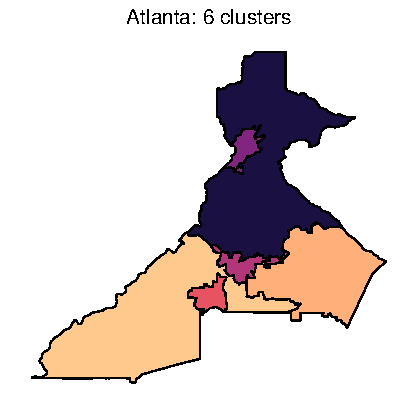
\includegraphics[width = .5\textwidth]{figs/Atlanta_clusters_binary_6.pdf} 
		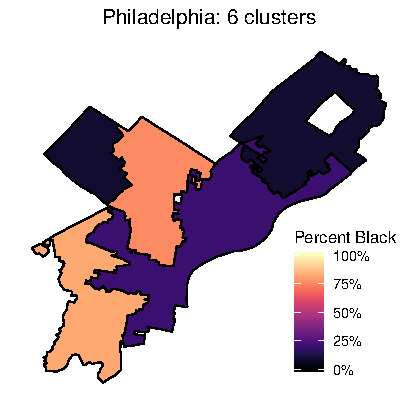
\includegraphics[width = .5\textwidth]{figs/Philadelphia_clusters_binary_6.pdf} \\
		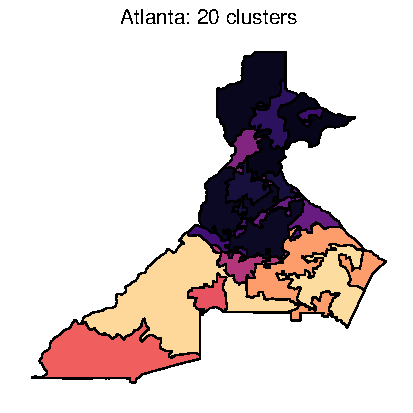
\includegraphics[width = .5\textwidth]{figs/Atlanta_clusters_binary_20.pdf}
		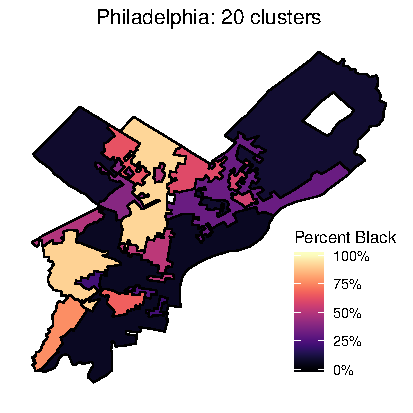
\includegraphics[width = .5\textwidth]{figs/Philadelphia_clusters_binary_20.pdf} \\
		
		\centering
		\begin{tabular}{l | c c c}
			\bfseries City  & $I(C_6, Y)$ & $I(C_{20},Y)$ & $I(X,Y)$ \\\hline
			\csvreader[late after line=\\]{figs/clustering_summary.csv}{}
			{\csvcoli & \csvcoliii & \csvcoliv & \csvcolii}
		\end{tabular}
		\caption{Example clusterings in Atlanta and Philadelphia using \eqref{eq:cluster_opt}, using $6$ and $20$ clusters. The table below summarizes the between-groups mutual information captured by each cluster and compares it to the mutual information in the unaggregated blockgroup level data.}

	\end{figure}

	\subsection{Binary Segregation Structure in Atlanta and Philadelphia}
		To demonstrate this approach for data analysis, we again compare black and non-black sociospatial trends in Atlanta and Philadelphia. While these two cities have similar spatial unevenness as measured by the mutual information $I(X,Y)$, the structure of this unevenness is very different. Because of a stark North-South divide in Atlanta, a simple clustering into six regions captures the vast bulk of sociospatial structure, conveying 0.28 nats out of a possible .34. In contrast, capturing a similar proportion of sociospatial structure in Philadelphia requires 20 clusters, reflecting the substantially more complex pattern of sociospatial variation. 

		The clusters found by these method may be viewed as coarse-grained views of the city that discard small details and leave only the high-level patterns. Comparison with the unaggregated data in Figure \ref{fig:Atlanta_philly} shows that the aggregate pictures highlight patterns of variation that may not be visible to the naked eye. Not every such cluster corresponds to a sociologically meaningful area or phenomenon, and care by the analyst is required in choosing an appropriate number of clusters. 

	\subsection{Structure of Multigroup Segregation in Detroit}
		\begin{figure}
		\centering
			\begin{subfigure}[b]{0.45\textwidth}
			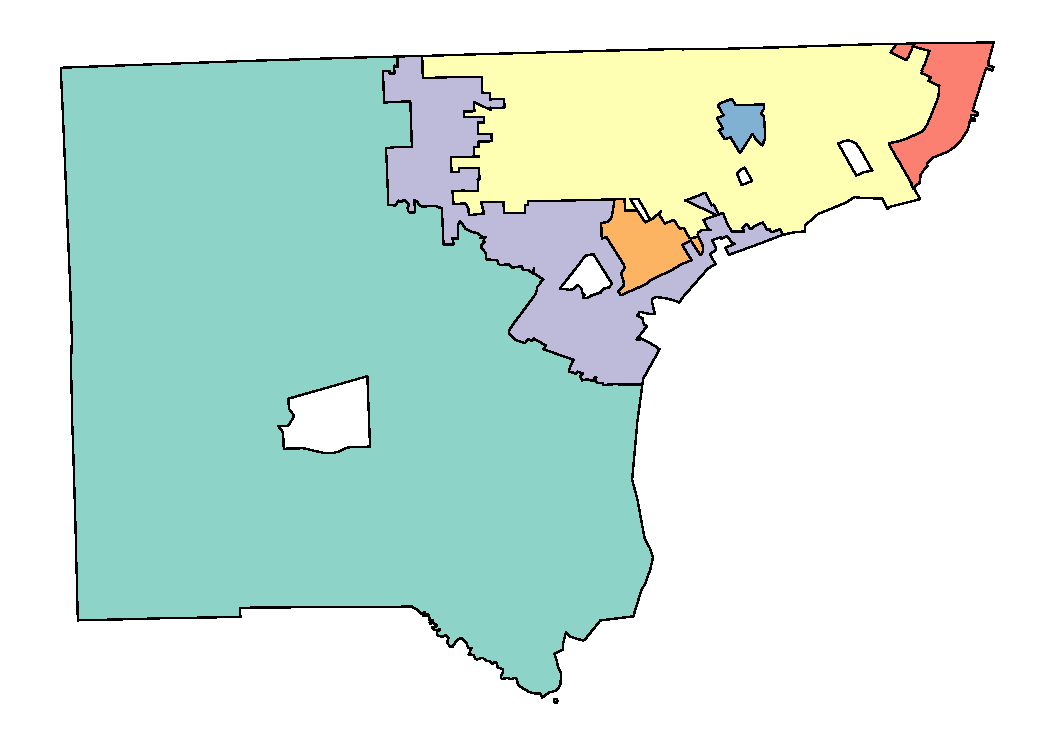
\includegraphics[width = \textwidth]{figs/example_cluster_map.pdf}
			\caption{} \label{subfig:detroit_map}
			\end{subfigure}
			\begin{subfigure}[b]{0.45\textwidth}
			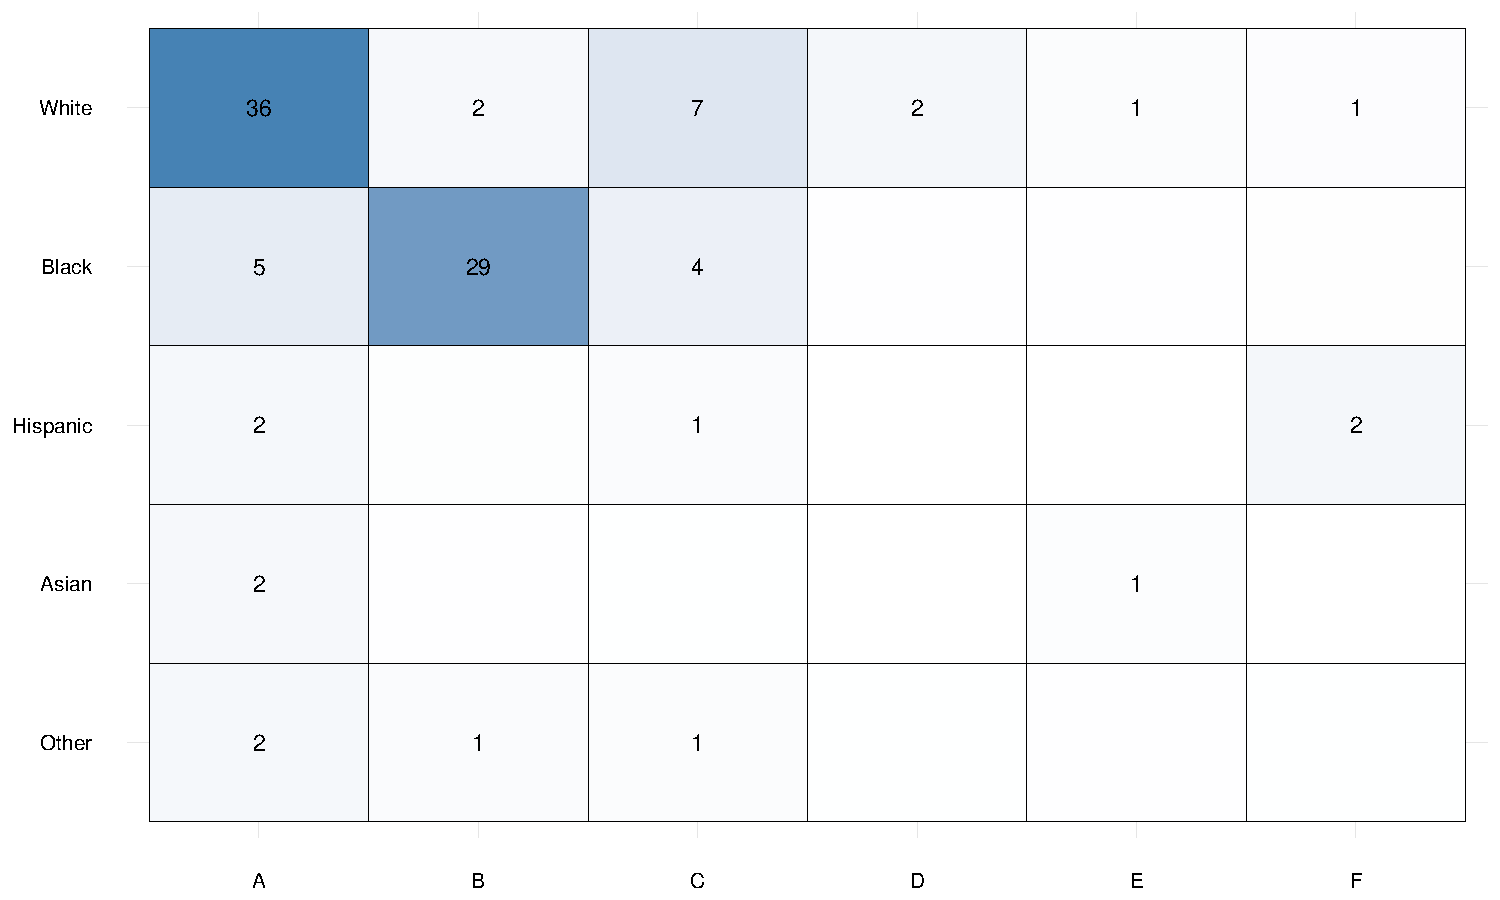
\includegraphics[width = \textwidth]{figs/example_clusters_detailed.pdf}
			\caption{} \label{subfig:detroit_groups}
			\end{subfigure}
			\caption{Multigroup sociospatial structure in Detroit. \ref{subfig:detroit_map}: Map of six clusters. \ref{subfig:detroit_groups}: Joint distribution of demographics and clusters. Shadings reflect population proportions within clusters. Numerical labels give raw population proportions; for example, 29\% of the population is Black and resides in cluster B. Detroit has $H(Y) = 1.12$, $I(X,Y) = 0.57$, and $J(X,Y) = 0.08$. This clustering captures $I(C_6,Y) = 0.36$ nats of information.} \label{fig:detroit}
		\end{figure}

		This technique extends naturally to multi-group settings, though the visualization of results requires more subtlety. In Figure \ref{fig:detroit}, we conduct an illustrative analysis of multigroup segregation segregation in Detroit and the surrounding Wayne County. The prominent clusters A and B reflect the primary white/black division in the city, with A representing the white suburbs and B the denser black inner city. Cluster C is interpretable as a transitional area between these two populations, with both white and black residents represented. Cluster D coincides with the historically distinct, predominantly white town of Grosse Pointe. Cluster E coincides with the city of Hamtramck, whose history has been shaped by high levels of immigration from Europe and Asia. Finally, Cluster F coincides with the Hispanic neighborhood Mexicantown. 

		Aside from simply highlighting geographic trends, this analysis also enables the quantitative study of traditional concerns in segregation studies, such as concentration. According to \cite{Massey1988}, ``\emph{concentration} refers to the degree of a group's agglomeration in urban space.'' The concept of concentration invites us to consider the composition and density of each cluster. For example, whites make up 70\% of ``their'' cluster A, while black residents make up 86\% of ``their'' cluster B. Cluster B is also more densely populated than Cluster A: it contains 34\% of Wayne County's population, but just 19\% of the analyzed geographic area, making it more than twice as dense as Cluster A. Thus, in and around Detroit, black neighborhoods tend to be both more racially homogeneous and more densely packed in urban space than white ones. We can also learn about pairwise group exposure. For example, from Figure  \ref{subfig:detroit_groups}, we observe that Asian residents tend to be found alongside white residents, but more rarely alongside black or Hispanic residents. Hispanic residents tend to group in Mexicantown and in predominantly white neighborhoods -- not black ones.

	\subsection{Relation of Clusterings and Information Measures}

		As discussed, the mean local information $J(X,Y)$ can be viewed as a measure of the number and character of transitional areas between regions of differing demographic structure.  It is low in Atlanta because the city is dominated by one, large North-South boundary while it is higher in Philadelphia due to many points of contact between neighborhoods of differing composition. Sociospatial transitions are also precisely the ``fault lines'' along which we would expect the clustering algorithm \eqref{eq:cluster_opt} to split the city. It is therefore not a coincidence that Philadelphia both has a higher value of $J(X,Y)$ and requires a greater number of clusters to convey a similar amount of sociospatial information. 

		To quantify the relationship between the mean local information $J(X,Y)$ and the clustering method \eqref{eq:cluster_opt}, we must first quantify the performance of the latter. We can do this by considering the number of clusters necessary to convey a given fraction of overall mutual information. Consider the between-groups information $I(C_N,Y)$ plotted as a function of the number $n$ of clusters. The result is a curve reflecting how information changes at varying levels of aggregation. Figure \ref{fig:AUC} shows examples of these curves for Atlanta, Detroit, and Philadelphia, with $N$ plotted on a logarithmic scale. The area under the curve (AUC) serves a measure of how early information is ``captured'' by the clustering. When the AUC is high, small numbers of clusters suffice to capture most of the information; when it is low more complex clustering is necessary. The AUC can be computed explicitly via the formula
		\begin{figure}
			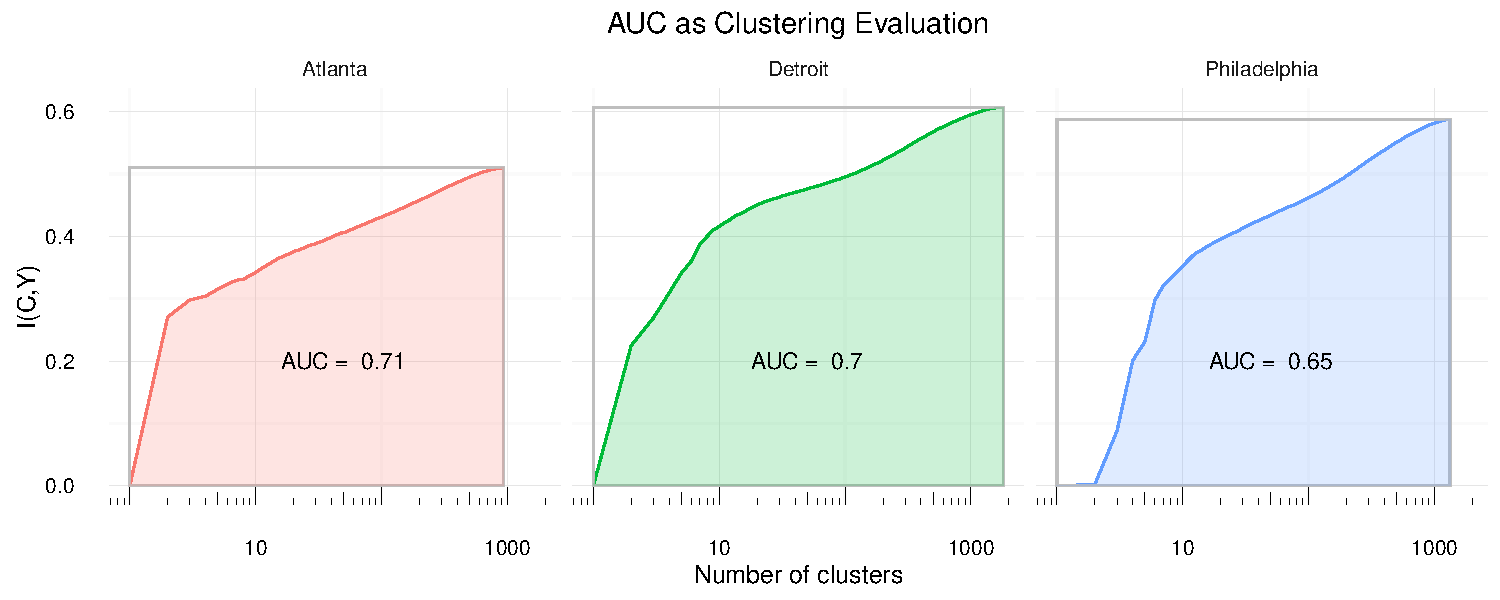
\includegraphics[width=\textwidth]{figs/AUC_illustration.pdf}
			\caption{Evaluation of clusterings using the area under the curve (AUC) for $\mathcal{Y} = \{\text{Black }, \text{Non-Black}\}$, computed according to the formula \eqref{eq:AUC_formula}. The bounding rectangle for each city is shown in grey. The AUC is the proportion of the rectangle contained in the shaded region. The AUC for Philadelphia has been adjusted to account for the data set's two disconnected geographic components.} \label{fig:AUC}
		\end{figure}
		\begin{equation}
			AUC = \frac{1}{I(X,Y) \log N} \sum_{n=1}^N I(C_n, Y) \log \frac{n+1}{n}, \label{eq:AUC_formula}
		\end{equation}
		and is shown overlaid in Figure \ref{fig:AUC}. 

		Comparing the three cities we have discussed so far, Atlanta and Detroit have relatively high AUC, indicating that that simple models with few clusters suffice to convey most of the sociospatial information in those cities. This can be interpreted physically as the existence of a small number of contiguous, starkly-separated regions, such as the North-South divide in Atlanta (cf. Figure \ref{fig:Atlanta_philly}). Philadelphia in contrast has a lower AUC, indicating that more complex models with more clusters are necessary to capture an equivalent amount of information. 

		\begin{figure}
			\centering
			\input{figs/adjusted_regression.txt}
			\caption{Regression of the AUC computed by \eqref{eq:AUC_formula} on the information measures $H(Y)$, $I(X,Y)$, and $J(X,Y)$. 95\% confidence intervals for each of the determined coefficients are shown in parentheses. The three information measures jointly explain an adjusted 75\% of the variation in the AUC. Table produced using \cite{Marek2015}.}\label{fig:regression}
		\end{figure}

		AUC is therefore an algorithmic measure of sociospatial complexity, which is high when there are few sociospatial boundaries and low when there are many. Previously, we also argued that the quantities $H(Y)$, $I(X,Y)$, and $J(X,Y)$ may be viewed as information measures of sociospatial complexity, and particularly that $J(X,Y)$ measures the presence of sociospatial boundaries. We should therefore expect that these two sets of measures are related. A simple way to test for the relationship is via linear least squares regression. We aim to approximate the AUC via the formula
		\begin{equation*}
			AUC \approx m_1H(Y) + m_2I(X,Y) + m_3J(X,Y) + b\;.
		\end{equation*}
		The results of this approximation are shown in Figure \ref{fig:regression}. Collectively, the three information measures suffice to explain an adjusted 75\% of the variation in the AUC, confirming that both the information measures and the algorithmic AUC measure the same underlying sociospatial structure. The coefficients are also instructive. The largest magnitude by far is the coefficient of $I(X,Y)$; all else equal, clustering is more effective when groups are distributed unevenly. The negative sign on the coefficient of the mean local information $J(X,Y)$ confirms our specific expectations from above; for fixed $I(X,Y)$ and $H(Y)$, a city with higher $J(X,Y)$ (more sociospatial complexity) is more difficult to model or simplify than one with lower $J(X,Y)$. 

\section{Discussion} \label{sec:discussion}
<<<<<<< HEAD
BLAH BLAH BLAH
% \bibliography{/Users/phil/bibs/library.bib}{}
% \bibliographystyle{plain}
=======

	We have developed a multidimensional, computationally practical, and mathematically unified approach to measuring residential segregation. An ensemble of three information measures -- the entropy $H(Y)$, mutual information $I(X,Y)$, and mean local information $J(X,Y)$ -- lie at the heart of this approach. These three measures jointly comprise an ensemble of measures corresponding to global diversity, spatial evenness, and spatial exposure. All three measures have operational interpretations in the context of predictive guessing games, and all may be computed easily from freely-available Census data. Furthermore, we have presented an information-based method for algorithmically identifying the high-level spatial structure of segregation, and related the performance of this algorithm to our core ensemble of information measures. We discuss two topics in this concluding section. First, we consider approaches to further improving these measures through spatial preprocessing of the underlying data. Second, we discuss the broader applicability of our information-theoretic framework to further problems both within and beyond segregation studies. 

	\subsection*{Areal Units, Anisotropy, and Spatial Preprocessing}

		The information measures developed here take their data (provided by the Census) as ``given,'' and compute with it directly. Two criticisms may be justly leveled against this approach. First, the demarcations of Census areal units are to some extent arbitrary: changing them would not change the underlying demographic phenomena, but may change the values of the mutual information or local information. This is a case of what is often called the ``modifiable areal unit problem,'' or MAUP \cite{Openshaw1981}. Second, using these areal units directly takes no notice of the intrinsically anisotropic nature of urban systems: two neighborhoods may be no more than 50 meters away, but if they are separated by a river, they may be functionally ``farther'' from each other than two other neighborhoods 500m apart \cite{Roberto2015}. In \cite{Roberto2015}, Roberto suggests a way to address both of these criticisms. Instead of computing with the data distributions $p(Y|X)$ of demographics at locations $X$, use instead the processed distributions $\bar{p}(Y|X)$, where 
		\begin{equation}
				\bar{p}(Y = y|X = x) \triangleq \frac{\int p(Y = y,X = \xi)\phi(x, \xi) d\xi}{\int p(X = \xi)\phi(x, \xi) d\xi}\;, \label{eq:divergence_smoother}
		\end{equation} 
		The function $\phi:M\times M \rightarrow \R_+$ is a spatial kernel that can be specified by the analyst. In the original formulation, the spatial kernel is the \emph{biweight proximity} given by 
		\begin{equation*}
			\phi(x, \xi) \triangleq 
			\begin{cases} 
				\left[1 - \frac{\delta(x, \xi)^2}{r^2} \right]^2 & \text{if } \delta(x, \xi) < r \\
				0 & \text{otherwise\;},
			\end{cases}
		\end{equation*}
		where $\delta:M\times M \rightarrow \R_+$ measures distance between two locations. 

		The processed distributions $\hat{p}(Y|X)$ may be regarded as having been \emph{smoothed} according to the kernel $\phi$. Appropriate smoothing can address both MAUP and anisotropy. With respect to MAUP, smoothing may be viewed as a way of robustifying measures by averaging out noise induced by arbitrarily demarcated areal units. With respect to anisotropy, the specific choice of the kernel $\phi$ is up to the analyst, and there is no requirement that it reflect the standard Euclidean distance. Roberto demonstrates proximity function that depends on road distance, implicitly reflecting anisotropy induced by infrastructure distributions and geographic boundaries. 

		Roberto goes on to compute a Divergence Index at each location $X$ according to the formula 
		\begin{equation*}
			DI(X) \triangleq D[\bar{p}(Y|X)\|p(Y)] 
		\end{equation*}
		and an overall Divergence Index 
		\begin{equation}
			DI \triangleq \E_X[DI(X)]. \label{eq:divergence_index} 
		\end{equation}
		Simple algebra may be used to express \eqref{eq:divergence_index} in the form 
		\begin{equation*}
			DI = D[\bar{p}(X,Y) \| p(X)\bar{p}(Y)]. 
		\end{equation*}
		Comparing to \eqref{eq:info_and_divergence}, we can recognize the the Divergence Index as a form of the mutual information with spatial preprocessing. A similar preprocessing approach may be used to calculate a modified local information; simply replace $p(Y|X)$ with $\hat{p}(Y|X)$ in all formulae. It may be that this preprocessing approach offers a substantial improvement to both measures. Further experiments on the numerical impact of MAUP and anisotropy are called for in order to determine whether these benefits justify the additional computational costs and analytical degrees of freedom associated with specifying $\phi$.  


	\subsection*{Local Information as a Complexity Measure}

		We have developed the local information $J_Y(X)$ as a measure of spatial exposure contextualized by the mutual information. As discussed briefly, another way to view the local information is as a measure of \emph{intrinsic sociospatial complexity}. Cities with high mean local information, such as Philadelphia, have more complex spatial structure than those with low mean local information such as Atlanta. Urban complexity has been a lively topic of interest at the intersection of physics and urban planning. Physically, the complexity of cities can be viewed as a rough measure of the complexity of theories needed to explain their structure and dynamics \cite{Bettencourt2015}. From a planning perspective, the complexity of land use was famously theorized by Jane Jacobs \cite{Jacobs1992} to be a driver of the health of neighborhoods. This theory has received preliminary empirical support \cite{DeNadai2016a}, with more tests no doubt to come. The local information can capture local variations in land use as well as demographics. We hope that this measure will serve as a useful tool for scholars of urban spatial complexity.  


	\subsection*{Generalizations and Further Applications}

		As noted above, the utility of our information-theoretic framework is not restricted to the study of residential racial segregation. The same methods may be used for studying other demographic variables distributed in space, such as income, education level, and occupation type. They may also be used for studying non-demographic phenomena, such as land use and infrastructure distributions. Considering this generality, it is tempting to also generalize these measures to handle two or more demographic variables simultaneously, enabling joint analysis of, for example, race and income. Unfortunately, this generalization is nontrivial. The core difficulty lies in generalizing the mutual information to multiple variables. Most formulations of multivariate mutual information have the challenging property that they may be negative, leading to difficulties of interpretation.  Substantial progress has been made on this front in the three-variable case by Loet Leydesdorff and collaborators \cite{Leydesdorff2014,Leydesdorff2015,Leydesdorff2013}, but generalized intuition on how to measure relations between multiple random variables remains elusive. 

		A simpler and no less useful generalization relates to temporal dynamics. A major challenge for information theory in urban science is the development of principled dynamical models that can explain observed information measures \cite{Batty2014a}. One approach to this challenge is to observe how information changes over time at varying scales. On the timescale of decades, information measures may be used to analyze the evolution of the evolving sociospatial structure of cities. Information-maximizing agglomerative clustering could then be used to cluster coherent regions in time as well as space, enabling a view of shifting demographic boundaries.

		Another avenue of exploration is on the much shorter timescale of daily mobility. Many adults spend less than half of their waking hours at home \cite{BureauofLaborStati2014}, indicating that residential segregation is only a partial characterization of city-wide diversity. Fortunately, our ability to learn about daily patterns of human mobility is progressing at a rapid pace. Recent years have seen an enormous increase in the use of mobile devices, allowing the passive collection of digital traces. These traces can be processed, analyzed, and validated to derive insight into daily activity patterns \cite{Widhalm2015,Yang,Jiang2013,Jiang2012c}. By combining these traces with residential demographics, it is possible to estimate flows of different demographic groups throughout the city on a daily basis. 

\bibliography{/Users/phil/bibs/library.bib}{}
\bibliographystyle{plain}
>>>>>>> 5f104e78623861e80c09faadeeae9579d0cc0598

\section*{Appendix}
	\subsection*{Software}
		We are pleased to make available two software repositories accompanying this analysis. 
		  \begin{itemize}
		    \item Package \texttt{compx} for the \texttt{R} programming language implements computation of the information measures $H(Y)$, $I(X,Y)$, and $J(X,Y)$, as well as a method for information-theoretic clustering. Access \texttt{compx} at 
		    \begin{displayquote}
		      \texttt{https://github.com/PhilChodrow/compx}. 
		    \end{displayquote}
		    To install in \texttt{R}, install the package \texttt{devtools} at 
		    \begin{displayquote}
		    \texttt{https://cran.r-project.org/web/packages/devtools/index.html}
		    \end{displayquote}
		     and run the command 
		    \begin{displayquote}
		      \texttt{devtools::install\_github(``PhilChodrow/compx'')}
		    \end{displayquote}
		    in the \texttt{R} console. 
		    \item The analysis repository for this project, including data acquisition and processing; core computations; and figure generation. We hope that this repository will provide useful examples of how to use \texttt{compx} for others aiming to replicate and extend our results. Download the project files at 
		    \begin{displayquote}
		      \texttt{https://github.com/PhilChodrow/spatial\_complexity}. 
		    \end{displayquote}
		  \end{itemize}

	\subsection*{Data and Methods}

	\begin{itemize}
		\item \textbf{Access}: All data used in this study are freely available from the U.S. Census. The \texttt{R} packages \texttt{acs} and \texttt{tigris} were used to programmatically download demographics and geographic shapefiles, respectively.
		\item \textbf{Specification:} All demographic data is from the Five-Year Estimates of the 2014 American Community Survey, Table B03002. 
		\item \textbf{Selection of Geographic Areas:} The delimiting of cities based on non-arbitrary population densities or natural boundaries is an area of active discussion in urban planning. For recent advances, see \cite{Rozenfeld2008,Rozenfeld2011}. W took a simple approach for the purposes of this study. For each city considered, we analyzed the region composed of all (and only those) counties in which some or all of the city's municipal boundaries lie. For example, our region corresponding to Atlanta consists of Fulton and Dekalb Counties, our region corresponding to Philadelphia consists of Philadelphia County, and the region corresponding to Detroit consists of Wayne County. For independent cities such as Baltimore and Washington D.C., the region of analysis consists simply of the municipal city boundaries. 
		\item \textbf{Aggregation of Racial Categories:} The data provided by Table B03002 contains categories corresponding to two options for ethnicity (Hispanic or Latino, Not Hispanic or Latino) and nine corresponding to race, giving a total of 18 cross-tabulated categories. For the purposes of analysis, we aggregated these into just five categories, \{\text{Asian}, \text{Black}, \text{Hispanic}, \text{Other}, \text{White}\}. The correspondence used is given in the GitHub repository \texttt{PhilChodrow/spatial\_complexity} linked above, under \texttt{assumptions/race\_lookup.csv}. 
		\item \textbf{Analysis and Visualization:} All analysis and visualization was conducted in the \texttt{R} statistical programming language. We used \cite{Bivand2014b,Bivand2014a,Bivand2014} for geographic analysis, and \cite{Wickham} for visualization.
	\end{itemize}

		

	\subsection*{Relationship of Mutual and Fisher Informations}

	Let $X$ be a continuous random variable taking values in $\R^n$, and let $Y$ be a discrete random variable define on finite alphabet $\mathcal{Y}$. Suppose further that $p(y|x) > 0$ and that $p(y|x)$ is differentiable as a function of $x$ for all $x,y \in \R^n \times \mathcal{Y}$. Fix $x_0 \in \R^n$, and define $B_r \triangleq B_r(x_0) = \{ x \in R^n \;|\; \norm{x - x_0} \leq r \}$. Additionally, define the \emph{local mutual information} in $B_r$ as the mutual information between $X$ and $Y$ where $X$ is restricted to $B_r$:
		\begin{align*}
			I_r(x_0) &\triangleq \E_X[D[p(\cdot|X)\| p(\cdot|X \in B_r)]|X \in B_r] \\
			&= \int_{B_r} p(x|X \in B_r) D[p(\cdot|x)\| p(\cdot|X \in B_r)] d^n x\;.
		\end{align*}
		where $D[p\|q] \triangleq \sum_{y} p(y) \log \frac{p(y)}{q(y)}$ is the Kullback-Leibler divergence of $q$ from $p$. 

		\begin{thm} \label{thm1}
			Under the stated conditions, 
			\begin{equation*}
				\lim_{r\rightarrow 0} \frac{I_r(x_0)}{r^2} = \frac{n}{2(n+2)} \emph{trace}\; J_Y(x_0)\;.
			\end{equation*}
			where the Fisher information matrix $J_Y$ is given by 
			\begin{align*}
			J_Y(x) &\triangleq \E_Y\left[\nabla_x S_{Y}(x)\nabla_x S_{Y}(x)^T \right] \\
			S_y(x) &\triangleq \log p(y|x)\;.
		\end{align*}
		\end{thm}

	We first define the following functions. For set $A$, let 
	\begin{equation*}
		f_A(x) \triangleq  D[p(y|x) \| p(y|x\in A)] \;.
	\end{equation*}
	Additionally, let 
	\begin{align*}
		q_r(x) &\triangleq p(x|X \in B_r)\;.
	\end{align*}
	We can then write the local mutual information as 
	\begin{equation*}
		I_r(x_0) = \int_{B_r} q_r f_{B_r} \; d\lambda\;,
	\end{equation*}
	where $\lambda$ is the Lebesgue measure in $\R^n$. We also let $V_r \triangleq \int_{B_r} \; d\lambda$ be the volume of $B_r$. Finally, define 
	\begin{equation*}
		a_r(y) \triangleq p(X \in B_r, Y). 
	\end{equation*}

	\begin{lm}
		For all $x \in B_r$,  
		\begin{equation*}
			q_r(x) = \frac{1 + O(r)}{V_r}\;.	
		\end{equation*}
	\end{lm}
	\begin{proof}
		First, Taylor's theorem implies that there exists a linear map $T$ such that 
		\begin{align*}
			p(x) &= p(x_0) + T(x - x_0) + O(\norm{x - x_0}^2) \\
			&= p(x_0) + T(x - x_0) + O(r^2)\;. 
		\end{align*}
		 Then, 
		\begin{align*}
			p(X\in B_r) &= \int_{B_r} p \; d\lambda \\
			&= \int_{B_r} p(x_0) + T(x - x_0) + O(r^2) d^n x\;.
		\end{align*}
		The middle term vanishes by spherical symmetry, leaving 
		\begin{align*}
			p(X\in B_r) &= p(x_0)V_r  + O(r^{n+2})\;.
		\end{align*}
		For $x \in B_r$, we therefore have 
		\begin{align*}
			p(x|X \in B_r) &= \frac{p(x,X \in B_r)}{p(X \in B_r)} \\ 
			&= \frac{p(x)}{p(X \in B_r)} \\
			&= \frac{p(x_0) + T(x - x_0) + O(r^2)}{p(x_0)V_r  + O(r^{n+2})} \\
			&= \frac{p(x_0) + O(r) + O(r^2)}{p(x_0)V_r} \\
			&= \frac{1 + O(r)}{V_r}\;,
		\end{align*}
		as was to be shown. 
	\end{proof}

	\begin{lm}
		For all $y\in Y$,
		\begin{equation*}
			a_r(y) = p(x_0,y)V_r + O(r^{n+2})\;.
		\end{equation*}
	\end{lm}
	\begin{proof}
		Taylor's Theorem again implies that, for any $(x,y)\in B_r \times \mathcal{Y}$, there is a linear map $T$ such that
		\begin{align*}
			p(x,y) &= p(x_0,y) + T(x - x_0) + O(\norm{x - x_0}^2) \\
			&= p(x_0,y) + T(x - x_0) + O(r^2). 
		\end{align*}
		We then have 
		\begin{align*}
			p(X \in B_r, y) &= \int_{B_r} p(x,y) \; d^n x \\ 
			&= \int_{B_r} p(x_0,y) + T(x - x_0) + O(r^2) \; d^n x \\
			&= p(x_0,y)V_r + O(r^{n+2}) \; d^n x\;,
		\end{align*}
		where the middle term has again vanished due to spherical symmetry. 
	\end{proof}
	\begin{lm}
		For any $y \in \mathcal{Y}$, we have $p(y|X \in B_r) = p(y|x_0) + e_y$, where the error terms $e_y$ satisfy $e_y \in O(r^2)$ and $\sum_{y \in \mathcal{Y}} e_y = 0$. 
	\end{lm}
	\begin{proof}
		That the errors must satisfy $\sum_{y \in \mathcal{Y}} e_y = 0$ follows from the fact that $p(\cdot| X \in B_r)$ must be a valid probability distribution on $\mathcal{Y}$. We'll now show that $e_y \in O(r^2)$. We then have 
		\begin{align*}
			p(y|X \in B_r) &= \frac{p(X \in B_r, Y)}{p(X\in B_r)} \\
			&= \frac{p(x_0, y)V_r + O(r^{n+2})}{p(x_0)V_r + O(r^{n+2})} \\
			&= p(y|x_0)  O(r^{2}) \tag{$V_r \propto r^n$}\;,
		\end{align*}
		as needed. 
	\end{proof}
	\begin{lm}
		For any $x \in B_r$, 
		\begin{equation*}
			f_{B_r}(x) = f_{x_0}(x) + O(r^3)\;.
		\end{equation*}
	\end{lm}
	\begin{proof}
		We compute directly: 
		\begin{align*}
			f_{B_r}(x) &= D[p(\cdot|x)\|p(\cdot|X \in B_r)] \\
			&= \sum_{y\in \mathcal{Y}} p(y|x) \log \frac{p(y|x)}{p(y|X \in B_r)} \\
			&= \sum_{y\in \mathcal{Y}} p(y|x) \log p(y|x) - \sum_{y \in \mathcal{Y}} p(y|x) \log p(y|X \in B_r)\; \\
			&= \sum_{y\in \mathcal{Y}} p(y|x) \log p(y|x) - \sum_{y \in \mathcal{Y}} p(y|x) \log (p(y|x_0) + e_y) \\ 
			&= \sum_{y\in \mathcal{Y}} p(y|x) \log p(y|x) - \sum_{y \in \mathcal{Y}} p(y|x) \log p(y|x_0) + \frac{e_y}{p(y|x_0)} + O(e_y^2)   \\
			&= \sum_{y\in \mathcal{Y}} p(y|x) \log p(y|x) - \sum_{y \in \mathcal{Y}} p(y|x) \log p(y|x_0) + \sum_{y\in \mathcal{Y}} \frac{p(y|x)}{p(y|x_0)}e_y + O(e_y^2) \\
			&= D[p(\cdot|x)\|p(\cdot|x_0)] + \sum_{y\in \mathcal{Y}} \frac{p(y|x)}{p(y|x_0)}e_y + O(e_y^2) \\
			&= f_{x_0}(x) + \sum_{y\in \mathcal{Y}} \frac{p(y|x)}{p(y|x_0)}e_y + O(e_y^2)\;.
		\end{align*}
		It remains to show that the error term is of order $O(r^3)$. Invoking Taylor's Theorem again, there exists a linear map $T$ such that 
		\begin{align*}
			\sum_{y\in \mathcal{Y}} \frac{p(y|x)}{p(y|x_0)}e_y + O(e_y^2) &= \sum_{y\in \mathcal{Y}} \left(1 +  \frac{1}{p(y|x_0)} T(x - x_0) + O(\norm{x - x_0}^2) \right)e_y + O(e_y^2) \\
			&= \sum_{y\in \mathcal{Y}} \left(1 +  O(r) + O(r^2) \right)e_y + O(e_y^2) \\
			&= \sum_{y\in\mathcal{Y}}\left[e_y + O(r^3)\right] \\
			&= O(r^3)\;, 
		\end{align*}
		since $\sum_{y\in \mathcal{Y}} e_y = 0$ by the previous lemma. 
	\end{proof}

	We now invoke the following well-known theorem of information geometry; for reference see \cite{Amari2000}. 

	\begin{thm}
		The Kullback-Leibler divergence and Fisher information $J_Y$ are related according to the following approximation: 
		\begin{equation*}
			D[p(\cdot|x)\|p(\cdot|x_0)] = \frac{1}{2} \left<x - x_0, J_Y(x_0)(x - x_0)\right> + O(\norm{x - x_0}^3)\;. 
		\end{equation*}
	\end{thm}

	Theorem 2 allows us to write $I_r(x_0)$ as the following spherical integral: 

	\begin{align*}
		I_r(x_0) &= \int_{B_r} q_r f_{B_r} \; d\lambda \\ 
		&= \int_{B_r} q_r(x) f_{B_r}(x_0)\; d^n x \\
		&= \int_{B_r} \frac{1 + O(r)}{V_r} \left(f_{x_0}(x) + O(r^3)\right) \; d^n x \\
		&= \frac{1 + O(r)}{V_r} \int_{B_r} \left(f_{x_0}(x) + O(r^3)\right) \; d^n x \\
		&= \frac{1}{2}\frac{1 + O(r)}{V_r} \int_{B_r} \left( \left<x - x_0, J_Y(x_0)(x - x_0)\right>  + O(r^3)\right) \; d^n x \\ 
		&= \frac{1}{2}\frac{1 + O(r)}{V_r} \left(\int_{B_r}  \left<x - x_0, J_Y(x_0)(x - x_0)\right> d^n x + V_rO(r^3)\right). 
	\end{align*}
	It remains to compute the integral, which we do using the following lemma: 

	\begin{lm} For any positive-semidefinite matrix $A \in \R^{n\times n}$, 
			$$\int_{B_r} \left< x - x_0, A(x-x_0) \right> d^n x = \frac{n}{n+2} r^{2} V_r \text{\emph{trace}} (A)$$
	\end{lm}
		
	\begin{proof}
		Since $A$ is positive-semidefinite, there exist an orthonormal matrix $P$ and a diagonal matrix $D$ such that $A = P^TDP$. Furthermore, the entries of $D$ are the eigenvalues $\{\lambda_i\}$ of $A$. Then, 
		\begin{align*}
			\int_{B_r} \left< x - x_0, A(x-x_0) \right> d^n x &= \int_{B_r} \left< x - x_0, P^T DP(x-x_0) \right> d^n x\\
			&= \int_{B_r} \left< P(x - x_0),  DP(x-x_0) \right> d^n x \;.
		\end{align*}
		We can regard $P$ as a reparameterization of $B_r$; since $\det P = 1$, we have 
		\begin{align*}
			\int_{B_r} \left< P(x - x_0),  DP(x-x_0) \right> d^n x &= \int_{B_r} \left< x - x_0,  D(x-x_0) \right> d^n x \\
			&= r^n\int_{B_n} \left< rx, rDx \right> d^n x \\
			&= r^{n+2}\int_{B_n} \left< x, Dx \right> d^n x \;,
		\end{align*}
		where $B_n$ is the unit $n$-ball. We also let $S_n(r)$ be the $n$-sphere of radius $r$. Continuing, 
		\begin{align*}
			r^{n+2}\int_{B_n} \left< x, Dx \right> d^n x &= r^{n+2} \int_{B_n} \sum_{i= 1}^n x_i^2 \lambda_i \; d^nx \\
			&= r^{n+2} \sum_{i = 1}^n \lambda _i \int_{B_n} x_i^2 \; d^nx \\
			&= \frac{r^{n+2}}{n} \sum_{i = 1}^n \lambda _i \int_{B_n} \norm{x}^2 \; d^nx \tag{spherical symmetry} \\
			&= \frac{r^{n+2}}{n} \text{tr}(A)  \int_{B_n} \norm{x}^2 \; d^nx \\ 
			&= \frac{r^{n+2}}{n} \text{tr} (A) \int_{\rho \in [0,1]} \rho^2 S_{n-1}(\rho) d\rho \\
			&= \frac{r^{n+2}}{n} \text{tr} (A) \int_{\rho \in [0,1]} \rho^{n+1} S_{n-1}(1) d\rho \\
			&= \frac{r^{n+2}}{n} \text{tr} (A)  \frac{1}{n+2} S_{n-1}(1) \\
			&= \frac{r^2}{n+2}  \text{tr} (A)  n r^{n}v(B_n(1)) \\
			&= \frac{n}{n+2} r^{2} V_r \text{tr} (A)\;,
		\end{align*}
		as was to be shown. 
	\end{proof}

	We may therefore complete the proof: 

	\begin{align*}
		I_r(x_0) &= \frac{1}{2}\frac{1 + O(r)}{V_r} \left(\int_{B_r}  \left<x - x_0, J_Y(x_0)(x - x_0)\right> d^n x + V_rO(r^3)\right) \\ 
		&= \frac{1}{2}\frac{1 + O(r)}{V_r} \left[\frac{n}{n+2} V_r \text{tr } J_Y(x_0) + V_rO(r^3)\right] \\
		&= r^2 \frac{n}{2(n+2)} \left(1 + O(r)\right)\left[\text{tr }J_Y(x_0) + O(r^3) \right]\;.
	\end{align*}
	Dividing through by $r^2$ and taking the limit as $r\rightarrow 0$ proves the theorem.	 

\end{document}